\documentclass{article}
\usepackage[utf8]{inputenc}

\title{Combustion HW-3}
\author{}
\date{}


\usepackage{graphicx}

\begin{document}

\maketitle

\section{Estimate the flame thickness}
Laminar flame speed 
$$
S_L=\frac{(2Le\int_{T_u}^{T_b} (T_b-T)ce^{-E/RT}dT)^{1/2}}{{\rho}_u\sqrt{\frac{c_p}{\lambda}}(T_b-T_u)}
$$
Flame thickness
$$
l_F=\frac{(\lambda/c_p)|_{Tref}}{\rho_uS_L}
$$

(a) the $CH_4-O_2$ flame\\
$CH_4:\ \lambda_{CH_4}=0.034\ W/m\cdot K$, $\rho_{CH_4}=0.657\ kg/m^3$, $c_{p,CH_4}=2.23\ kJ/kg\cdot K$\\
$O_2:\ \lambda_{O_2}=0.026\ W/m\cdot K$, $\rho_{O_2}=1.308\ kg/m^3$, $c_{p,O_2}=0.92\ kJ/kg\cdot K$\\
$Mixture:\ \lambda=0.0276\ W/m\cdot K$, $\rho=1.178\ kg/m^3$, $c_p=1.18\ kJ/kg\cdot K$\\
for $CH_4-O_2$ case, typically $S_L=0.3\ m/s$, therefore:
$$
l_{F,CH_4}=0.066\ mm
$$

(b) the $H_2-O_2$ flame\\
$H_2:\ \lambda_{H_2}=0.1848\ W/m\cdot K$, $\rho_{H_2}=0.082\ kg/m^3$, $c_{p,H_2}=14.3\ kJ/kg\cdot K$\\
$O_2:\ \lambda_{O_2}=0.026\ W/m\cdot K$, $\rho_{O_2}=1.308\ kg/m^3$, $c_{p,O_2}=0.92\ kJ/kg\cdot K$\\
$Mixture:\ \lambda=0.0436\ W/m\cdot K$, $\rho=1.172\ kg/m^3$, $c_p=2.41\ kJ/kg\cdot K$\\
for $H_2-O_2$ case, typically $S_L=3.0\ m/s$, therefore:
$$
l_{F,H_2}=0.005\ mm
$$


\section{Review the derivation of the burning velocity}
Governing equations:
$$
\dot{m} \frac{dY_i}{dx}=D\rho \frac{d^2Y_i}{dx^2} - \omega
$$
$$
\dot{m} c_p \frac{dT}{dx}=\lambda \frac{d^2T}{dx^2} + Q \omega
$$
where $\omega = B_cYe^{-T_a/T}$ (the dependence of $\omega$ on the  parameters and the concentration are absorbed in $B_c$)\\
Non-dimensional form:
$$
\frac{d^2\tilde{T}}{d\tilde{x}^2} - \frac{d\tilde{T}}{d\tilde{x}} = -\frac{B_c}{c_p\dot{m}^2/\lambda}\tilde{Y}e^{-E/R\tilde{T}}
$$
$$
\frac{d^2\tilde{T}}{d\tilde{x}^2}+\frac{1}{Le}\frac{d^2\tilde{Y}}{d\tilde{x}^2}-\frac{d(\tilde{T}+\tilde{Y})}{\tilde{x}}=0
$$
where $\tilde{T}=c_pT/q_cY_u$, $\tilde{Y}=Y/Y_u$ and $\tilde{x}=c_px/\dot{m}\lambda$

In the non-reaction zone, reaction rate $\omega$ is approximately zero, while in the reaction zone, the first order derivative can be safely neglected. Integrate from $-\infty\ to\ 0$ and $0\ to\ \infty$ respectively under this assumption:
$$
\frac{d^2\tilde{T}}{d\tilde{x}^2} - \frac{d\tilde{T}}{d\tilde{x}} = 0
$$
$$
(\frac{d\tilde{T}}{d\tilde{x}})^2=2Le\frac{B_c}{c_p\dot{m}/\lambda}\int_{\tilde{T_0}}^{\tilde{T_b}} (\tilde{T}_b-\tilde{T})e^{-E/R\tilde{T}}d\tilde{T}
$$
at x=0, these two solutions need to be consistent, which means:
$$
\tilde{T}_b-\tilde{T}_u = [2Le\frac{B_c}{c_p\dot{m}/\lambda}\int_{\tilde{T_0}}^{\tilde{T_b}} (\tilde{T}_b-\tilde{T})e^{-E/R\tilde{T}}d\tilde{T}]^{1/2}
$$
in dimensional form:
$$
\dot{m}(T_b-T_u)\sqrt{c_p/\lambda}=[2Le\int_{T_0}^{T_b} (T_b-T) c e^{-E/RT}dT]^{1/2}
$$
where $\dot{m}=\rho_uS_L$. Substitute this into the above equation yields the burning velocity:
$$
S_L=\frac{[2Le\int_{T_0}^{T_b} (T_b-T) c e^{-E/RT}dT]^{1/2}}{{\rho}_u\sqrt{\frac{c_p}{\lambda}}(T_b-T_u)}
$$

$S_L$ is dependent on $T_b$ (adiabatic flame temperature), while $T_b$ is related to $\phi$ (equivalence ratio) as discussed in HW-I. Therefore, $S_L$ reaches its maximum at $\phi=1$. However, under practical conditions, the maximum point will shift a little to $\phi>1$.


\section{Nonadiabatic thermal explosion}
The energy conservation equation can be written as:
$$
\rho_0c_v\frac{dT}{dt}=-Q_c\frac{dc_F}{dt}-Sh(T-T_0)=Q_c B c_F exp(-T_a/T)-Sh(T-T_0)
$$
With $\tilde{T}=(c_v \rho_0 / Q_c c_{F,0})T=(c_v/q_cY_{F,0})T$ and $\tilde{c}_F = c_F/c_{F,0}$, the above equation becomes:
\begin{equation}
   \frac{d\tilde{T}}{dt}=-\frac{d\tilde{c}_F}{dt}-\frac{Sh}{c_v\rho_0}(\tilde{T}-\tilde{T}_0)=B \tilde{c}_F exp(-\tilde{T}_a/\tilde{T})-\frac{Sh}{c_v\rho_0}(\tilde{T}-\tilde{T}_0)
\end{equation}

Assume that the temperature is perturbed from its initial value by a small amount,
$$
\tilde{T}=\tilde{T}_0 + \epsilon \theta(t) + O(\epsilon^2)
$$
where $\theta(0)=0$ and $\epsilon=\tilde{T}_0^2/\tilde{T}_a \ll 1$. Substitute the temperature perturbation relation into Equation 1, and neglect reactant consumption during the induction period, the temperature perturbation $\theta$ is governed by:
\begin{equation}
   \frac{d\theta}{d\tilde{t}}=e^\theta - \tilde{h}\theta 
\end{equation}
where $\tilde{h}=\tau_c/\tau_L$, and $\tau_L=c_v\rho_0/(hS/V)$


\section{Ignition/extinction problem}

(1) The temperature equation\\
Overall energy balance for a given mass flow rate $\dot{M}$ in steady state:
$$
\dot{M}c_p(T_f-T_0)=VQ_cBc_Fe^{-T_a/T_f}
$$
using $\tilde{T}_f-\tilde{T}_0=1-\tilde{c}_F$, the above equation can ba expressed in non-dimensional form as
$$
\tilde{T}_f-\tilde{T}_0=Da(\tilde{T}_{ad} - \tilde{T}_f) e^{-\tilde{T}_a / \tilde{T}_f}
$$
where $\tilde{T}=(c_p/q_cY_{F,0})T$, $Da=BV/\dot{M}$ being the Damkohler number, and $\tilde{T}_{ad}=a+\tilde{T}_0$ being the adiabatic flame temperature.\\

(2) The dependence of $\tilde{T}_f$ on $Da$\\
$$
\tilde{T}_f-\tilde{T}_0=Da(\tilde{T}_{ad} - \tilde{T}_f) e^{-\tilde{T}_a / \tilde{T}_f}
$$
Solve this equation numerically, and the result is shown in Figure \ref{fig:sCurve}.\\

\begin{figure}[htpb]
\centering
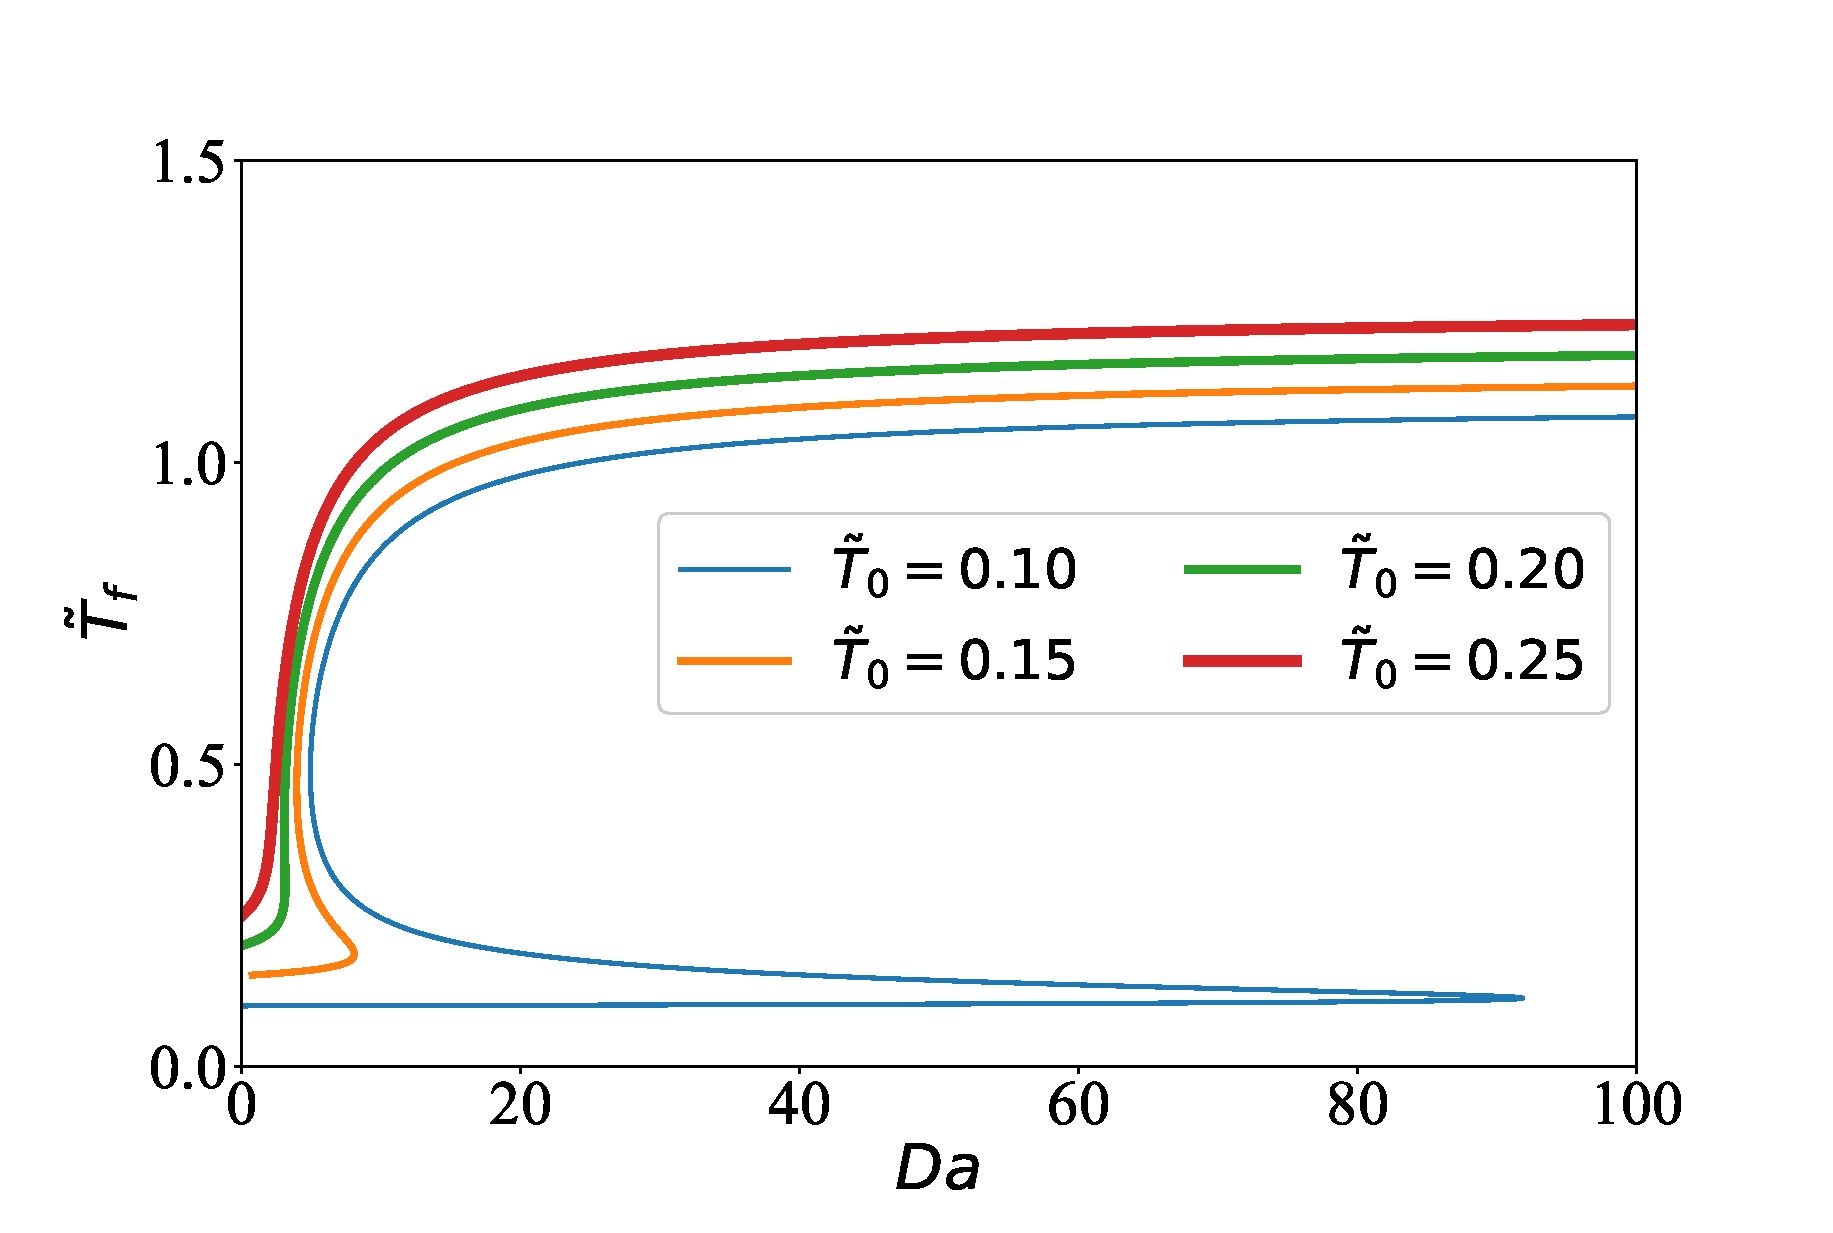
\includegraphics[scale=0.36]{sCurve.eps}
\caption{S-Curve}
\label{fig:sCurve}
\end{figure}

(3) The physics of ignition and extinction\\
By increasing the Damkohler number continuously along the S-Curve, we first cover all weakly reactive states. When $Da$ reaches $Da_I$, the system "jumps" to the upper branch, which exists for higher Damkohler numbers and faster reaction rates. Therefore point I can be identified as the state of ignition. Similarly, if moving along the upper branch with decreacing $Da$, the system will again jumps at point E back to the lower branch. This indicates the extinction state.


\end{document}
